\chapter{Testing}
Testing is a substantial part of the MangaVerse web application project. Testing helps to ensure application's 
reliability, performance and correctness. To be able to conduct efficient testing process, two kind of tests are preformed.
They are JUnit testing as a structural testing and functional testing.

\section{Structural Testing}
Structural testing also with other name white-box testing is based on testing the internal structure of the working application and it 
guarantees that the methods are working as expected.JUnit testing framework is used to conduct structural testing. JUnit testing is performed by testing 
different modules of the application such as DAOs and services. With that process each methods efficiency and correctness is guaranteed. 
Some examples of JUnit testing are shown below.\\ \\


\begin{figure}[h]
    \centering
    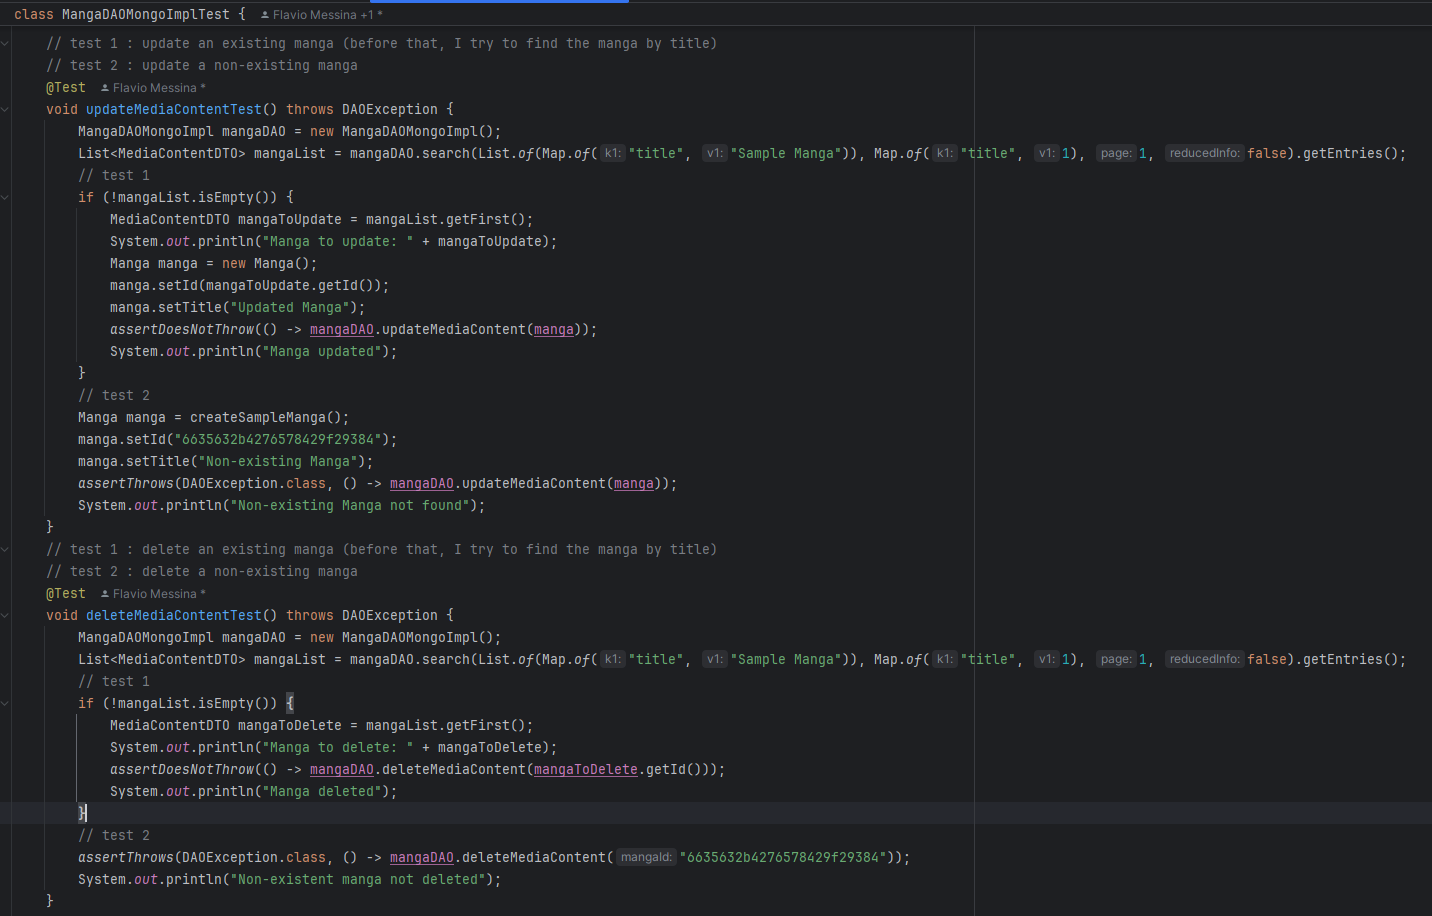
\includegraphics[width=\linewidth]{Media/test_example_1.png}
    \caption{MangaDAOMongoImpl Class Test Example}
    \label{MangaDAOMongoImpl Class Test Example}
\end{figure}

\begin{figure}[h]
    \centering
    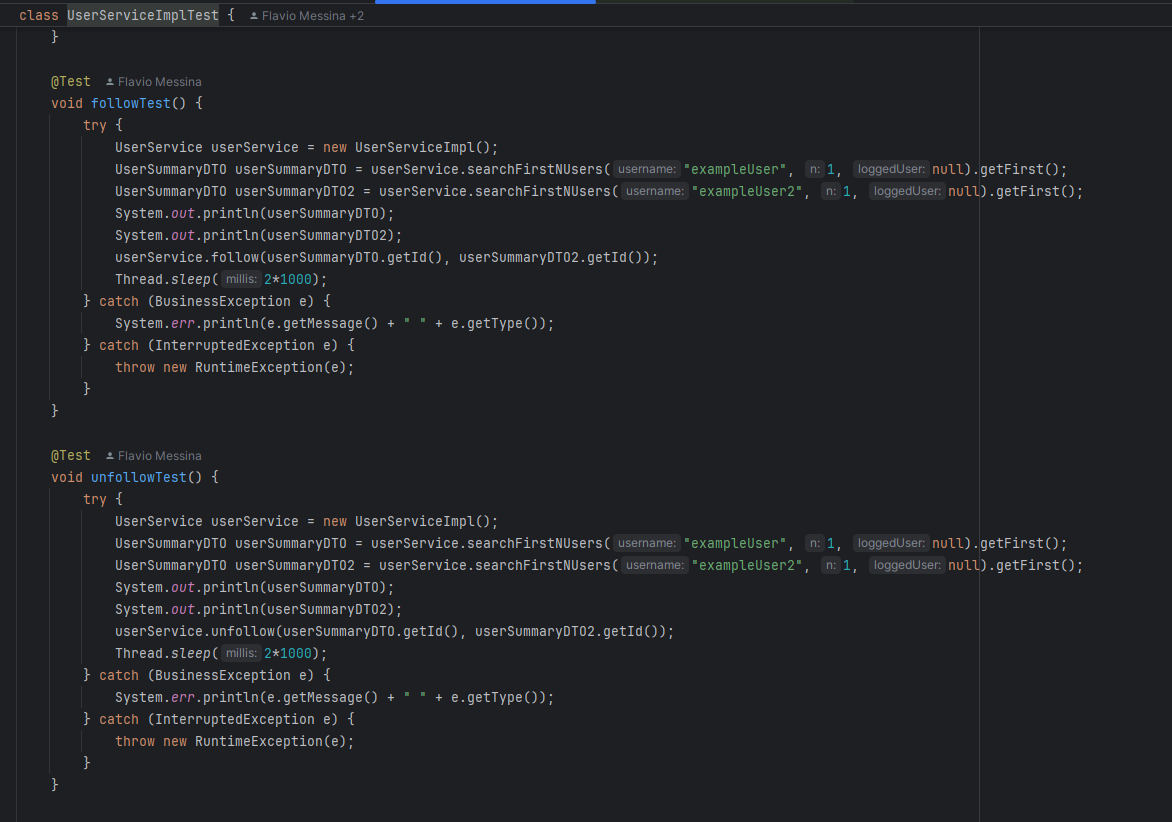
\includegraphics[width=\linewidth]{Media/test_example_2.png}
    \caption{UserServiceImpl Class Test Example}
    \label{UserServiceImpl Class Test Example}
\end{figure}

\newpage

\section{Functional Testing}
Functional testing also with other name black-box testing is based on testing the application's external functionalities. It checks the application from end-user's 
perspective. It ensures that specified requirements are provided efficiently by the web application and expected is outcome is created. 
With the help of the use cases and real world scenarios, functional testing is conducted. Some examples of functional testing are shown below.

